\documentclass[10pt,twocolumn]{article}

\usepackage[letterpaper,margin=0.85in,columnsep=0.28in]{geometry}
\usepackage{graphicx}
\usepackage{booktabs}
\usepackage{caption}
\usepackage{xcolor}
\usepackage{titlesec}
\usepackage{enumitem}
\usepackage[expansion=false]{microtype}
\usepackage[hidelinks]{hyperref}

\definecolor{secblue}{HTML}{2E5A88}
\definecolor{subblue}{HTML}{1F3A57}

\titleformat{\section}{\normalfont\large\bfseries\color{secblue}}{\thesection}{0.6em}{}
\titleformat{\subsection}{\normalfont\normalsize\bfseries\color{subblue}}{\thesubsection}{0.6em}{}
\titlespacing*{\section}{0pt}{10pt}{4pt}
\titlespacing*{\subsection}{0pt}{8pt}{3pt}

\captionsetup{font=small,labelfont=bf,textfont=it,skip=4pt}
\setlist[itemize]{leftmargin=1.1em,itemsep=1.5pt,topsep=3pt,parsep=0pt}
\setlength{\parskip}{3pt}
\setlength{\parindent}{0pt}
\renewcommand{\arraystretch}{1.15}

\title{\vspace{-1.4em}\textbf{\Large Faster Flow Simulations}\\[0.25em]
\normalsize\normalfont Multigrid solvers and reduced-precision arithmetic in OpenFOAM}

\author{\normalsize Shubh Chawda\\[0.15em]
\small BSc Computer Science, Year 1\\
\small University of Manchester}

\date{\small July 2026}

\begin{document}
\maketitle

\begin{abstract}
\noindent\small
Incompressible CFD is dominated by the cost of repeatedly solving a large
pressure system. This project measured two routes to reducing that cost on a
validated 2D laminar channel case: algebraic multigrid, and single-precision
arithmetic. Multigrid converts superlinear cost growth ($n^{1.51}$) into
near-linear ($n^{1.22}$) by keeping iteration counts nearly mesh-independent.
Single precision is shown to cost no accuracy where it converges (agreement to
$3\times10^{-7}$\,m/s) and to save 14--28\,\% of peak memory consistently, but
its speed effect \emph{reverses sign} with mesh size: 6.7\,\% faster at 16{,}384
cells, 31\,\% slower at 65{,}536. The controlling variable is not mesh size but
the fraction of pressure solves that exhaust the solver's iteration limit, which
rises as the single-precision convergence floor grows like $\sqrt{N}$. This
mechanism reconciles the present Apple Silicon measurements with an independent
Arm measurement of the opposite sign.
\end{abstract}

\section{Motivation and objective}

Computational fluid dynamics resolves a flow by dividing the domain into
millions of cells and solving the governing equations in each. It is accurate
but expensive, and for incompressible solvers the cost is dominated by one
repeated step: solving a large linear system for pressure at every timestep.
Reducing that cost is the difference between a simulation that takes hours and
one that takes days.

This project examined two ways of making that step cheaper, with a view to
eventually running on the Arm-based Isambard supercomputer:

\begin{itemize}
  \item \textbf{Better linear solvers} --- specifically algebraic multigrid
  (GAMG), designed to converge at a rate that does not degrade as the mesh is
  refined.
  \item \textbf{Reduced-precision arithmetic} --- 32-bit floats (fp32) instead
  of 64-bit doubles (fp64), halving the storage and memory traffic of every
  field.
\end{itemize}

The governing question was not simply ``is it faster?'' but ``how much faster
can this be made before the answer stops being trustworthy?'' --- which is why a
validated reference case was built before any optimisation was attempted.

\section{Method}

\textbf{Test case.} Two-dimensional laminar flow in a plane channel, solved with
OpenFOAM's \texttt{icoFoam}. Domain $1.0\times0.1\times0.01$\,m
(two-dimensionality imposed by a single cell in the spanwise direction with
\texttt{empty} patches), $\nu = 10^{-3}$\,m$^2$/s, uniform inlet of 1\,m/s,
no-slip walls. This gives $\mathrm{Re}_H = 100$, comfortably laminar. The case
was chosen because it has an exact analytical solution: the Poiseuille
parabola, peak velocity 1.5\,m/s, so every result can be checked against
theory rather than only against itself.

\textbf{Validation.} The developed outlet profile matches the analytical
solution to \textbf{0.08\,\% of peak velocity}, establishing a trusted baseline
before any solver or precision changes.

\textbf{Timing protocol.} Early timings were unusable: session-to-session drift
of ${\sim}1.85\times$ exceeded the effects being measured. All timings reported
here use a fixed protocol; identical timestep counts, three alternating
sequential repeats per precision, nothing else running, and median with spread
reported. Any claimed effect smaller than the observed spread is refused. For
the precision comparison a double-precision control was compiled from the
identical source tree, compiler and flags as the single-precision build, so that
the comparison measures precision rather than build differences (build effect
1.4\,\%, inside the 3.7\,\% spread).

\begin{figure*}[t]
  \centering
  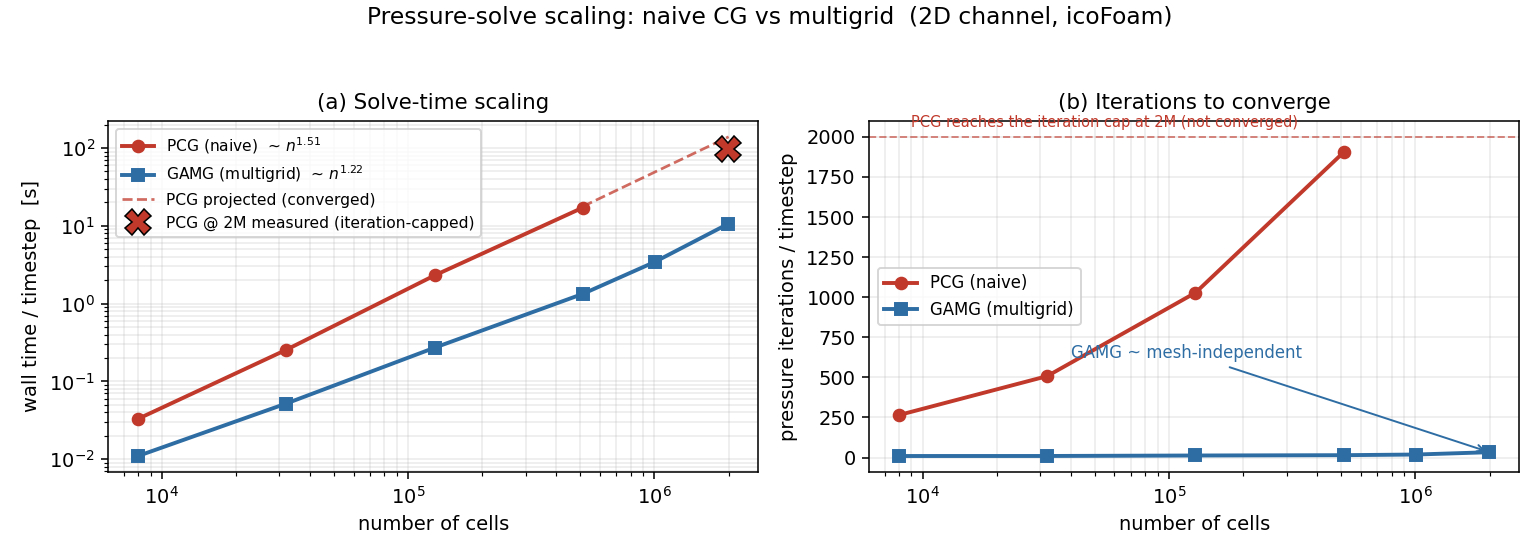
\includegraphics[width=\textwidth]{fig/scaling2.png}
  \caption{Pressure-solve scaling. Left: wall time per timestep against cell
  count. Right: iterations to converge --- PCG grows with the mesh, GAMG is
  close to mesh-independent.}
  \label{fig:scaling}
\end{figure*}

\section{Results}

\subsection{Multigrid changes the scaling law}

The same case was run from 8{,}000 to 2{,}000{,}000 cells with two pressure
solvers: preconditioned conjugate gradient (PCG) and algebraic multigrid (GAMG).
Fitted wall-time scaling with cell count gives PCG $\propto n^{1.51}$ and GAMG
$\propto n^{1.22}$ --- superlinear versus near-linear.

The mechanism is visible in the iteration counts (Fig.~\ref{fig:scaling}). PCG's
pressure iterations grow from 265 to 1{,}905 per timestep across the range,
because information must propagate across an ever-larger mesh; GAMG's rise only
from 10 to 33 over a $250\times$ increase in cells, because it removes
large-scale error cheaply on coarse grids. At 2 million cells GAMG solved at
${\sim}11$\,s per timestep; PCG, extrapolated from its fitted slope, would need
${\sim}2.3$ minutes per timestep, about $13\times$ longer.

\subsection{Mesh independence}

To identify the cheapest trustworthy mesh, the case was swept from 8{,}000 to
512{,}000 cells with the timestep scaled to hold the Courant number fixed, and
each mesh advanced to genuine steady state rather than a fixed end time.
Successive refinement changes the outlet centreline velocity by 0.094\,\%,
0.024\,\%, 0.004\,\% and 0.0015\,\% --- so the conventional 1\,\% criterion is
met even by the coarsest mesh and carries no information for this case. On a
0.01\,\% criterion, every output settles by roughly 128{,}000 cells.

Two checks confirm the solution is converging correctly rather than merely
settling. Self-convergence of the peak velocity gives an observed spatial order
of 2.0, matching the nominally second-order schemes. Separately, the error
against the analytical parabola falls but flattens onto a floor of
${\sim}0.018$\,\% of peak velocity; this is physical rather than numerical,
the outlet sits at twice the entrance length, so the flow is developed to about
99.98\,\%, not exactly. Subtracting that floor recovers clean second-order
convergence.

\begin{figure}[h]
  \centering
  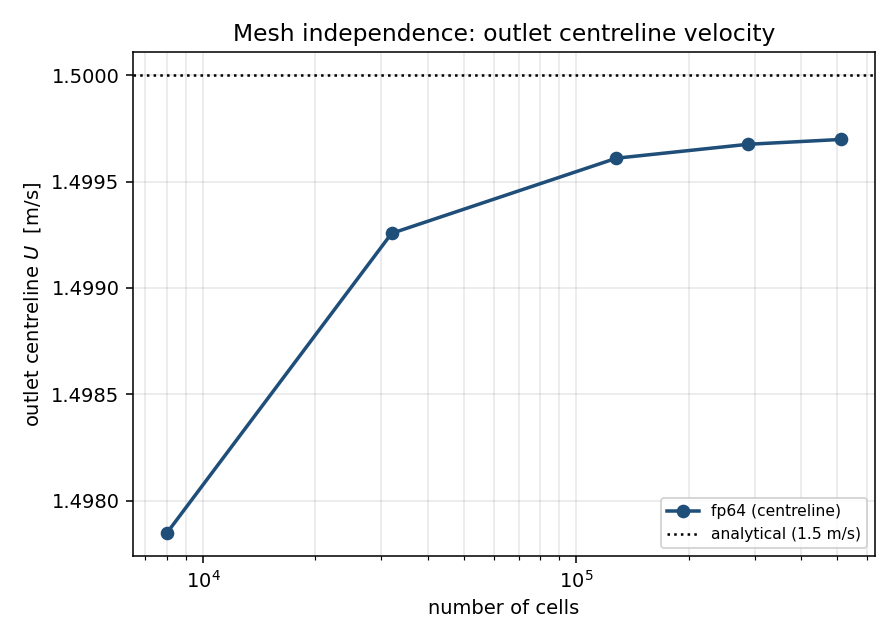
\includegraphics[width=0.94\columnwidth]{fig/convergence.png}
  \caption{Outlet centreline velocity against cell count, approaching the
  analytical 1.5\,m/s.}
  \label{fig:conv}
\end{figure}

\subsection{Single versus double precision}

Precision in OpenFOAM is a compile-time, whole-library setting, so this required
building a second, single-precision OpenFOAM from source. It is non-trivial on
macOS, requiring a case-sensitive filesystem (otherwise the C++ standard
library's \texttt{time.h} resolves to OpenFOAM's own \texttt{Time.H}) and the
correct link target for the OSspecific library.

\textbf{A prerequisite: a silent failure mode.} A collaborator at Arm identified a
mesh round-off bug in OpenFOAM's single-precision support: round-off in the
\texttt{empty}-patch face areas can exceed an internal threshold, causing $x$ and
$y$ to be marked as empty solution directions, after which the momentum
equations are skipped entirely --- while the run completes and produces
plausible output. Every fp32 log in this study was checked for the corresponding
solver lines; all were present, so these results are unaffected. Binary-exact
(power-of-two) cell counts were nonetheless used throughout the precision work,
since they cost nothing to adopt.

\textbf{Accuracy is not the issue.} Where both precisions converge, fp32 and
fp64 agree on peak outlet velocity to $3\times10^{-7}$\,m/s --- about
$2\times10^{-5}$\,\% of peak velocity --- with matching Courant numbers and
comparable continuity errors.

\textbf{Memory saving is consistent.} fp32 reduced peak resident memory by
13.6\,\% at 16{,}384 cells, 28.3\,\% at 65{,}536 cells, and 27.0\,\% for the PCG
comparison.

\textbf{Speed reverses sign with mesh size.} This was the central and unexpected
finding (Table~\ref{tab:speed}).

\begin{table*}[t]
  \centering
  \small
  \caption{Single- versus double-precision speed, GAMG, pressure tolerance
  $10^{-4}$. The 262{,}144-cell row is a \emph{work} comparison at a fixed
  tolerance target, not an accuracy-matched benchmark --- fp32 never reaches the
  tolerance there.}
  \label{tab:speed}
  \begin{tabular}{lccc}
    \toprule
    \textbf{Mesh (cells)} & \textbf{fp32 solves hitting the iteration cap} &
    \textbf{fp32 vs fp64 time} & \textbf{Repeats}\\
    \midrule
    16{,}384  & 0.00\,\%  & \textbf{6.7\,\% faster} & $n=3$ each\\
    65{,}536  & 0.20\,\%  & 31\,\% slower           & $n=3$ each\\
    262{,}144 & 95.31\,\% & $115.6\times$ slower\,$^{\dagger}$ & fp64 $n=2$, fp32 $n=1$\\
    \bottomrule
  \end{tabular}
\end{table*}

The governing variable is not mesh size but the fraction of pressure
solves that exhaust the solver's iteration limit. Single precision cannot drive
the pressure residual arbitrarily low; the achievable floor rises as roughly
$\sqrt{N}$, so on a fine enough mesh the solver can no longer reach the
requested tolerance and caps out. Each capped solve costs 1{,}000 iterations. At
65{,}536 cells just two capped solves out of 1{,}024 account for 55\,\% of
fp32's entire pressure workload; excluding them, the two precisions do
comparable work (1{,}636 versus 1{,}574 iterations). Per iteration fp32 is
consistently the cheaper of the two: 2.99 versus 3.46\,ms on the clean
16{,}384-cell comparison.

\begin{figure*}[t]
  \centering
  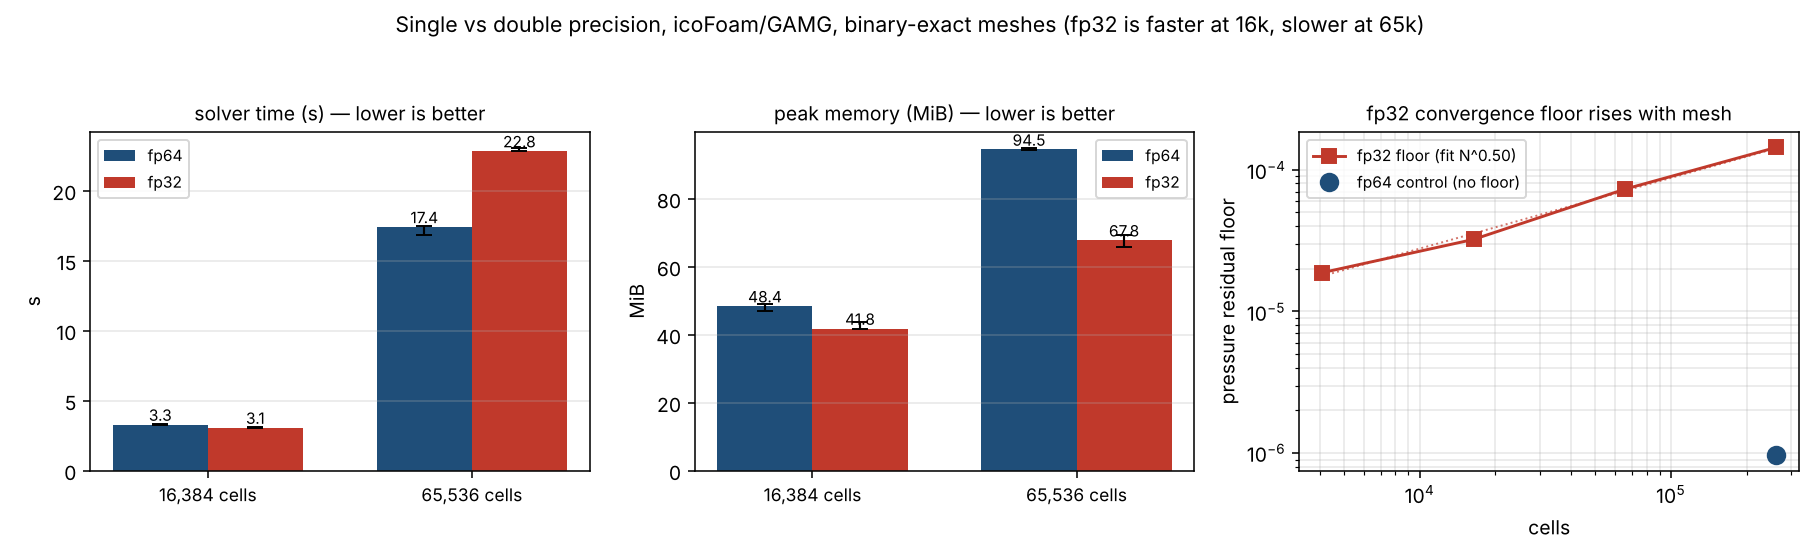
\includegraphics[width=\textwidth]{fig/fp32.png}
  \caption{Solver time, peak memory, and the rising fp32 convergence floor.
  fp32 is faster at 16k and slower at 65k; memory is lower in both.}
  \label{fig:fp32}
\end{figure*}

\begin{figure}[h]
  \centering
  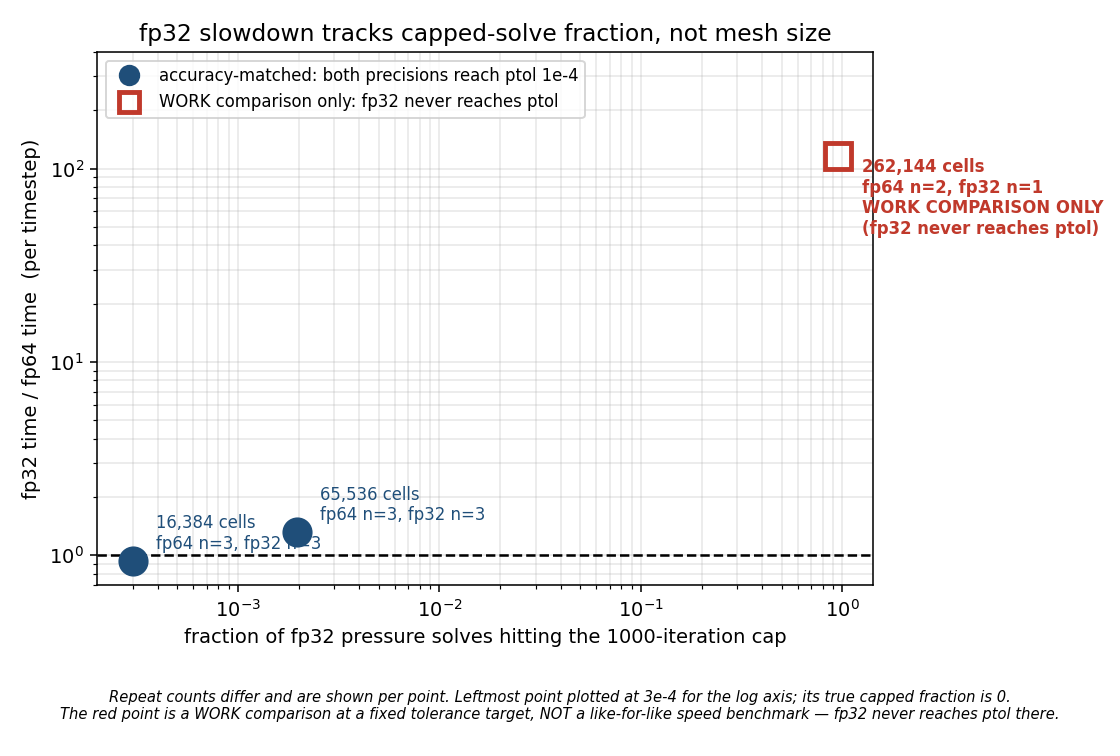
\includegraphics[width=0.94\columnwidth]{fig/capped.png}
  \caption{Relative fp32 speed against capped-solve fraction. The
  262{,}144-cell point (open square) is a work comparison at a fixed tolerance
  target, not an accuracy-matched benchmark.}
  \label{fig:capped}
\end{figure}

\textbf{PCG fails differently.} Repeating the comparison with PCG shows fp32 is
7.7\,\% slower and uses 27.0\,\% less memory --- but it never hits the iteration
cap. Instead it needs 9\,\% more iterations throughout, at essentially identical
per-iteration cost (1.22 versus 1.24\,ms). Both solvers therefore agree that
reduced precision costs \emph{iterations}, but by different routes: occasionally
and harshly for GAMG, mildly and steadily for PCG.

\textbf{Reconciliation with the Arm measurement.} A collaborator at Arm measured fp32 21.4\,\%
\emph{faster} on Arm; this study measured 31\,\% \emph{slower} on Apple Silicon
at 65{,}536 cells --- while both saw a substantial memory saving. These are
consistent under one mechanism: when the solver still reaches the requested
tolerance, fp32's cheaper arithmetic makes it faster; when it cannot, the capped
solves cost more than the arithmetic saves.
The memory benefit follows directly from halving field storage and is portable;
the speed benefit depends on solver, tolerance, mesh and hardware together, and
must be measured per platform.

\subsection{Inlet profiles}

Two further inlet conditions were run on the optimal mesh, bringing the
fluid-dynamics side of the problem to the optimised solver. An oscillating
inlet, $U(t) = 1 + 0.5\sin(2\pi t)$ at 1\,Hz (Womersley number
$\alpha \approx 4$), produced the expected unsteady signature: the outlet
centreline oscillates about the correct developed mean with visibly reduced
amplitude and a small, near-in-phase shift, because the profile cannot fully
re-develop within each cycle. The amplitude was deliberately chosen so the flow
never reverses --- the minimum velocity over the cycle was $+0.004$\,m/s,
confirming no backflow (Fig.~\ref{fig:inlets}, top).

A steady skewed inlet, peaking at one-third of the channel height, re-developed
fully to the symmetric parabola by the outlet (velocity centroid
$0.40 \rightarrow 0.50$ of channel height, outlet peak 1.5002), with the
asymmetry decaying below 0.5\,\% by $x \approx 0.44$\,m which is consistent with the
${\sim}0.5$\,m entrance length (Fig.~\ref{fig:inlets}, bottom).

\begin{figure}[htbp]
  \centering
  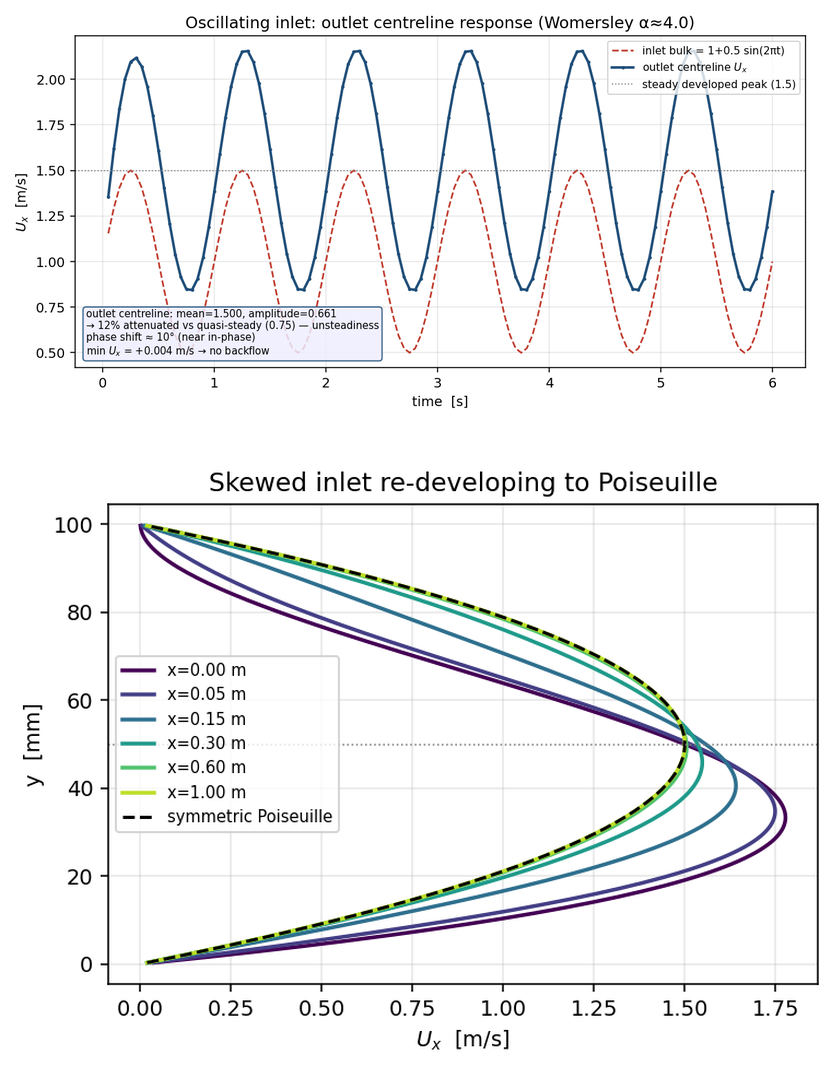
\includegraphics[width=0.95\columnwidth]{fig/inlets_stack.png}
  \caption{Inlet-profile cases. \textbf{Top:} oscillating inlet, outlet centreline
  response over six cycles at $\alpha \approx 4$ --- attenuated relative to the
  quasi-steady reference and everywhere positive, so no backflow.
  \textbf{Bottom:} skewed inlet, the asymmetric profile re-developing towards the
  symmetric Poiseuille parabola (dashed) along the channel.}
  \label{fig:inlets}
\end{figure}

\section{Conclusions}

\begin{itemize}
  \item \textbf{Multigrid is better.} GAMG converts superlinear cost
  growth ($n^{1.51}$) into near-linear ($n^{1.22}$) by keeping iteration counts
  almost independent of mesh size. This is what makes large meshes tractable at
  all.
  \item \textbf{Reduced precision does not cost accuracy here.} Where fp32
  converges, it agrees with fp64 to a few parts in ten million.
  \item \textbf{It reliably saves memory (14--28\,\%)} on every
  accuracy-matched comparison, in both solvers. This benefit is portable across
  platforms.
  \item \textbf{Its speed effect is conditional, not general.} It reverses sign
  with mesh size on one machine, and disagrees in sign between two machines. The
  controlling factor is whether the single-precision convergence floor forces
  the solver to cap, which depends on mesh, tolerance, solver and hardware
  together.
  \item \textbf{In practice:} full fp32 saves memory, but at a variable and
  sometimes severe cost to how far the solver can converge. That combination might point
  toward mixed precision, keeping the ill-conditioned pressure solve
  in double precision while doing cheaper work in single, rather than
  converting wholesale.
\end{itemize}

\section{Limitations}

\begin{itemize}
  \item One geometry throughout: a straight 2D channel on a uniform, orthogonal
  Cartesian mesh, laminar at $\mathrm{Re}_H = 100$, run serially. Five inlet
  conditions were tested (uniform, parabolic, pulsatile, oscillating and skewed),
  but the domain itself never changed --- no bends, expansions, obstacles or
  non-orthogonal cells, and nothing turbulent or three-dimensional. Complex
  geometries produce skewed meshes and recirculation that stress the pressure
  solver far harder, so these results should not be assumed to carry over.
  \item One machine for the precision study (Apple Silicon, Apple clang).
  Reduced-precision behaviour is hardware- and compiler-dependent; the
  Arm/Isambard target may behave differently, as the disagreement with the Arm
  measurement already shows.
  \item The speed crossover is bracketed between 16{,}384 and 65{,}536 cells but
  not located; a finer sweep would pin it.
  \item Repeat counts are $n=3$ per precision except at 262{,}144 cells
  (fp64 $n=2$, fp32 $n=1$), where the ${\sim}116\times$ effect far exceeds any
  plausible noise.
  \item The precision comparison uses a pressure tolerance of $10^{-4}$ rather
  than the $10^{-6}$ used elsewhere, because fp32 cannot reach $10^{-6}$ ---
  applied identically to both precisions.
\end{itemize}

\section{Further work}

\begin{itemize}
  \item \textbf{Mixed precision}, the natural response to the
  convergence-floor result, and the obvious next experiment.
  \item \textbf{Repeat on Isambard}, the target hardware, and where the
  speed result may differ; this needs its own single-precision build.
  \item \textbf{Locate the speed crossover} with a finer mesh sweep, and test
  whether tuning GAMG's coarsening offsets the precision floor.
  \item \textbf{Windows verification}, not attempted; requires a separate
  single-precision build.
\end{itemize}

\section*{Acknowledgements}
\small
I thank my supervisor at the University of Manchester, and the project's
collaborators at Arm and the University of Bath, for their guidance and input
throughout. The single-precision mesh round-off failure mode described in
\S3.3 was identified by a collaborator at Arm, whose independent measurement also
prompted the platform comparison. All case files, scripts and data are in the
project repository, together with the single-precision build recipe and a
verification check for the fp32 failure mode.

\end{document}
